\section{Deterministic Physics-Gate Ablation}
To isolate the value of physical feasibility filtering from the later robust-policy study, we compare two deterministic nominal selectors over the same 54-action space. Both use the same nominal communication/sensing QoS screen and the same normalized-resource ranking. The only difference is that the gated selector first applies the canonical range and unambiguous-velocity support test, whereas the ungated selector ranks all actions without that test. No Monte-Carlo uncertainty draws, Wilson bounds, or B4 reliability qualification are used in this Paper 1 ablation.

The operating grid is deliberately boundary-aware rather than probabilistically weighted. It contains 14 range values from 0 to 60 m and 17 signed radial-velocity values from $-60$ to $60$ m/s, including samples immediately around the parking and high-mobility support boundaries. Of the resulting 238 states, 132 are physically representable by at least one declared profile and 106 are outside the support of the complete action set.

% AUTO-GENERATED from Paper 1 physics-gate ablation evidence; do not hand-edit.
\begin{table}[t]
\centering
\caption{Paper-1 deterministic physics-gate ablation on the boundary-aware range--velocity grid.}
\label{tab:p1gateablation}
\begin{tabular}{lrrrr}
\toprule
Selector & Selected & Selection rate & Invalid & Invalid/selected\\
\midrule
Gated & 132 & 55.46\% & 0 & 0.00\%\\
Ungated & 238 & 100.00\% & 220 & 92.44\%\\
\bottomrule
\end{tabular}
\end{table}


The ungated selector returns an action in all 238 states, but 220 selections (92.44\%) violate the selected profile's deterministic range or velocity support. This percentage characterizes the deliberately boundary-stressing grid and must not be interpreted as a prevalence estimate for real driving. The gated selector selects in the 132 supportable states and makes zero physically invalid selections. In 114 states, the ungated selector chooses an invalid configuration even though another action in the same 54-action set is physically valid; the gate exposes that valid alternative before nominal QoS ranking. In the remaining unsupported states, gating correctly distinguishes physical infeasibility of the declared action set from policy abstention.

% AUTO-GENERATED from Paper 1 physics-gate ablation evidence; do not hand-edit.
\newcommand{\figPaperOneGateAblation}{%
\begin{figure*}[t]
\centering
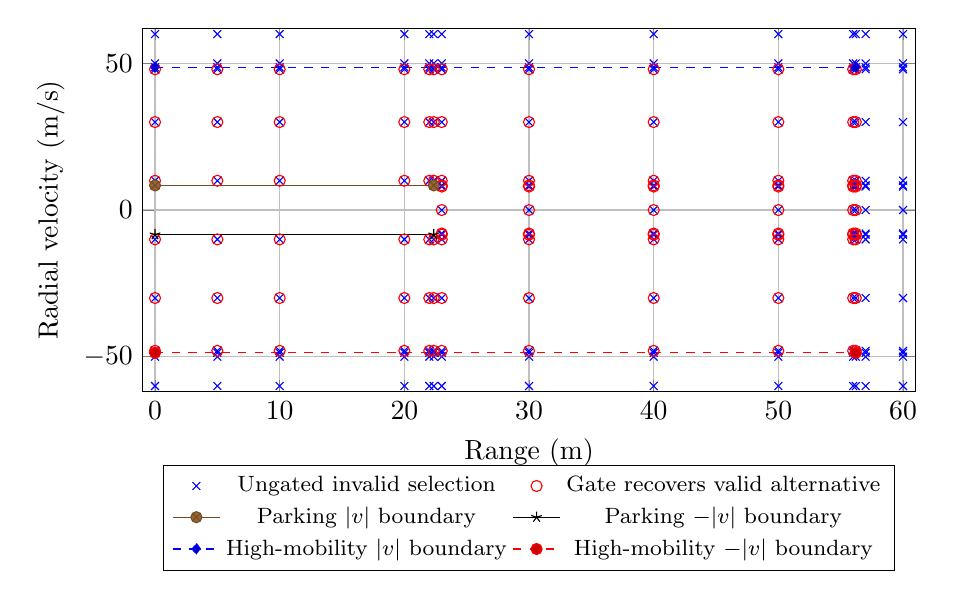
\begin{tikzpicture}
\begin{axis}[width=0.94\textwidth,height=6.2cm,xlabel={Range (m)},ylabel={Radial velocity (m/s)},xmin=-1,xmax=61,ymin=-62,ymax=62,grid=major,legend style={font=\footnotesize,at={(0.5,-0.20)},anchor=north,legend columns=2}]
\addplot+[only marks,mark=x] coordinates {(0,-60) (0,-50) (0,-48.67) (0,-48) (0,-30) (0,-10) (0,10) (0,30) (0,48) (0,48.67) (0,50) (0,60) (5,-60) (5,-50) (5,-48.67) (5,-48) (5,-30) (5,-10) (5,10) (5,30) (5,48) (5,48.67) (5,50) (5,60) (10,-60) (10,-50) (10,-48.67) (10,-48) (10,-30) (10,-10) (10,10) (10,30) (10,48) (10,48.67) (10,50) (10,60) (20,-60) (20,-50) (20,-48.67) (20,-48) (20,-30) (20,-10) (20,10) (20,30) (20,48) (20,48.67) (20,50) (20,60) (22,-60) (22,-50) (22,-48.67) (22,-48) (22,-30) (22,-10) (22,10) (22,30) (22,48) (22,48.67) (22,50) (22,60) (22.36,-60) (22.36,-50) (22.36,-48.67) (22.36,-48) (22.36,-30) (22.36,-10) (22.36,10) (22.36,30) (22.36,48) (22.36,48.67) (22.36,50) (22.36,60) (23,-60) (23,-50) (23,-48.67) (23,-48) (23,-30) (23,-10) (23,-8.41) (23,-8) (23,0) (23,8) (23,8.41) (23,10) (23,30) (23,48) (23,48.67) (23,50) (23,60) (30,-60) (30,-50) (30,-48.67) (30,-48) (30,-30) (30,-10) (30,-8.41) (30,-8) (30,0) (30,8) (30,8.41) (30,10) (30,30) (30,48) (30,48.67) (30,50) (30,60) (40,-60) (40,-50) (40,-48.67) (40,-48) (40,-30) (40,-10) (40,-8.41) (40,-8) (40,0) (40,8) (40,8.41) (40,10) (40,30) (40,48) (40,48.67) (40,50) (40,60) (50,-60) (50,-50) (50,-48.67) (50,-48) (50,-30) (50,-10) (50,-8.41) (50,-8) (50,0) (50,8) (50,8.41) (50,10) (50,30) (50,48) (50,48.67) (50,50) (50,60) (56,-60) (56,-50) (56,-48.67) (56,-48) (56,-30) (56,-10) (56,-8.41) (56,-8) (56,0) (56,8) (56,8.41) (56,10) (56,30) (56,48) (56,48.67) (56,50) (56,60) (56.21,-60) (56.21,-50) (56.21,-48.67) (56.21,-48) (56.21,-30) (56.21,-10) (56.21,-8.41) (56.21,-8) (56.21,0) (56.21,8) (56.21,8.41) (56.21,10) (56.21,30) (56.21,48) (56.21,48.67) (56.21,50) (56.21,60) (57,-60) (57,-50) (57,-48.67) (57,-48) (57,-30) (57,-10) (57,-8.41) (57,-8) (57,0) (57,8) (57,8.41) (57,10) (57,30) (57,48) (57,48.67) (57,50) (57,60) (60,-60) (60,-50) (60,-48.67) (60,-48) (60,-30) (60,-10) (60,-8.41) (60,-8) (60,0) (60,8) (60,8.41) (60,10) (60,30) (60,48) (60,48.67) (60,50) (60,60)};
\addplot+[only marks,mark=o] coordinates {(0,-48) (0,-30) (0,-10) (0,10) (0,30) (0,48) (5,-48) (5,-30) (5,-10) (5,10) (5,30) (5,48) (10,-48) (10,-30) (10,-10) (10,10) (10,30) (10,48) (20,-48) (20,-30) (20,-10) (20,10) (20,30) (20,48) (22,-48) (22,-30) (22,-10) (22,10) (22,30) (22,48) (22.36,-48) (22.36,-30) (22.36,-10) (22.36,10) (22.36,30) (22.36,48) (23,-48) (23,-30) (23,-10) (23,-8.41) (23,-8) (23,0) (23,8) (23,8.41) (23,10) (23,30) (23,48) (30,-48) (30,-30) (30,-10) (30,-8.41) (30,-8) (30,0) (30,8) (30,8.41) (30,10) (30,30) (30,48) (40,-48) (40,-30) (40,-10) (40,-8.41) (40,-8) (40,0) (40,8) (40,8.41) (40,10) (40,30) (40,48) (50,-48) (50,-30) (50,-10) (50,-8.41) (50,-8) (50,0) (50,8) (50,8.41) (50,10) (50,30) (50,48) (56,-48) (56,-30) (56,-10) (56,-8.41) (56,-8) (56,0) (56,8) (56,8.41) (56,10) (56,30) (56,48) (56.21,-48) (56.21,-30) (56.21,-10) (56.21,-8.41) (56.21,-8) (56.21,0) (56.21,8) (56.21,8.41) (56.21,10) (56.21,30) (56.21,48)};
\addplot+[domain=0:22.36,samples=2] {8.4055};
\addplot+[domain=0:22.36,samples=2] {-8.4055};
\addplot+[domain=0:56.21,samples=2,dashed] {48.6676};
\addplot+[domain=0:56.21,samples=2,dashed] {-48.6676};
\legend{Ungated invalid selection,Gate recovers valid alternative,Parking $|v|$ boundary,Parking $-|v|$ boundary,High-mobility $|v|$ boundary,High-mobility $-|v|$ boundary}
\end{axis}
\end{tikzpicture}
\caption{Boundary-aware Paper-1 ablation. Crosses mark states where the nominal ungated selector chooses a configuration outside its deterministic FMCW support; circles identify the subset for which physics gating instead exposes a valid alternative. Lines show the two profiles' unambiguous-velocity boundaries; range support is additionally enforced in the machine-readable evidence. This is deterministic analytical/simulation-model evidence, not a hardware measurement.}
\label{fig:p1gateablation}
\end{figure*}%
}

\figPaperOneGateAblation

The ablation therefore supports a narrow methodological claim: standard FMCW capability relations become operationally important when they are enforced as a hard first-stage constraint in finite-action configuration selection. It does not show that all ungated ISAC controllers fail, nor does it establish field reliability. Its purpose is to demonstrate a concrete selection failure mode that cannot be repaired by subsequent statistical averaging once an unsupported waveform has already been chosen.
